\chapter[Identificación de métodos builders]{Enfoques para la identificación de Métodos Builders}
\label{cap:builders}

El análisis de software es una tarea crucial en el campo de la Ingeniería de Software, ya sea para generar tests para el software bajo test (SUT)  o para realizar verificación de modelos de software. Estos enfoques requieren que los programadores identifiquen manualmente un subconjunto de los métodos de un módulo con el fin de dirigir el análisis. En general, al analizar un módulo, los programadores seleccionan un subconjunto de sus métodos que serán considerados como constructores de objetos (\emph{builders}) para definir lo que se conoce como un controlador o "driver", que se utilizará para construir objetos automáticamente para el análisis, combinándolos de manera no determinista, aleatoria, etc. Esto requiere una inspección minuciosa del módulo y su API, ya que la exhaustividad relativa del análisis (omitir métodos importantes puede evitar sistemáticamente la generación de diferentes objetos) y su eficiencia (las diferentes combinaciones acotadas de métodos crecen de manera exponencial a medida que aumenta el número de métodos) se ven afectados por la selección.

En este capitulo, proponemos tres enfoques para seleccionar automáticamente un conjunto de constructores de objetos a partir de la API de un módulo, basados en un algoritmo evolutivo y un algoritmo greedy y un algoritmo basado en clases de equivalencias. Estos algoritmos favorecen conjuntos de métodos cuyas combinaciones conducen a la generación de conjuntos más grandes de objetos o a aquellos conjuntos que obtienen mejor cobertura de ramas del SUT. Además, los algoritmos tienen en cuenta otras características de estos conjuntos de métodos, tratando de priorizar la selección de aquellos con menor cantidad de métodos y con más simples parámetros.

% Para evaluar experimentalmente nuestra propuesta, hemos realizado una evaluación en un conjunto de clases con estado de referencia, que representan casos de uso típicos. Los resultados muestran que nuestro enfoque puede identificar automáticamente conjuntos de constructores de objetos que son suficientes (se pueden utilizar para crear cualquier instancia del módulo) y mínimos (no contienen métodos superfluos), en un tiempo razonable.

% En resumen, en este trabajo abordamos el desafío de seleccionar automáticamente un conjunto óptimo de constructores de objetos a partir de la API de un módulo, con el objetivo de mejorar tanto la exhaustividad como la eficiencia del análisis de software. Nuestros resultados experimentales demuestran la viabilidad y efectividad de nuestra propuesta, lo que abre nuevas perspectivas para la automatización de la selección de constructores de objetos en el análisis de software.


\section{Motivacion}

\cacho{Change te order maybe. Explain in detalle en un solo lado}
\cacho{Los listing lo pongo como listing, como figure o como que para hacer referencia}

\begin{table}[H]
\center
{\scriptsize
\begin{tabular}{|l|l|l|l|}
\hline
No. &Return type & Method name & Obs? \\
\hline
    0 && NCL() & no \\
    1& & NCL(int) & no \\
    2&& NCL(Collection) & no \\
    3&boolean & add(Object) & no \\
    4&void&add(int,Object) & no \\
    5&boolean&addAll(Collection) & no\\
    6&boolean&addAll(int,Collection) & no \\
    7&boolean&addFirst(Object) & no \\
    8&boolean&addLast(Object) & no\\
    9&void&clear() & no\\
    10&boolean&contains(Object) & yes \\
    11&boolean&containsAll(Collection) & yes \\
    12&boolean&equals(Object) & yes \\
    13&Object&get(int) & yes\\
    14&Object&getFirst() &yes \\
    15&Object&getLast() & yes\\
    16&int&indexOf(Object) &yes\\
    17&boolean&isEmpty() & yes\\
    18&Iterator&iterator() & no\\
    19&int&lastIndexOf(Object) &yes \\
    20&ListIterator&listIterator() &no \\
    21&ListIterator&listIterator(int) & no\\
    22&Object&remove(int) &no\\
    23&boolean&remove(Object) & no \\
    24&boolean&removeAll(Collection) & no \\
    25&Object&removeFirst() &no\\
    26&Object&removeLast() &no\\
    27&boolean&retainAll(Collection) &no \\
    28&Object&set(int,Object) &no\\
    29&int&size() &yes\\
    30&List&subList(int,int) & no \\
    31&Object[]&toArray() & yes \\
    32&Object[]&toArray(Object[]) &yes\\
    33&String&toString() & yes \\
\hline
\end{tabular}
}
\caption{Apache's NodeCachingLinkedList API}
\label{tab:ncl-api}
\end{table} 
En esta sección, motivamos nuestro enfoque mediante un ejemplo práctico. La estructura de datos NodeCachingLinkedList (NCL) de Apache \cite{apache} consta de una lista doblemente enlazada circular principal que contiene los elementos de la colección y una lista secundaria simplemente enlazada que actúa como caché para los nodos que se han eliminado de la lista principal. Los nodos almacenados en la caché pueden ser reutilizados y añadidos de nuevo a la lista principal al insertar elementos en ella. Gracias a su caché, en las aplicaciones en las que las inserciones y eliminaciones de la lista son muy frecuentes, NCL puede reducir significativamente la sobrecarga necesaria para la asignación de memoria y la recolección de basura de los nodos. 
Como ilustración, la Figura~\ref{fig:ncl-instances} muestra las tres instancias de NCL que se pueden construir con exactamente dos nodos.


\begin{figure}[H]
    \centering
    
\includegraphics[width=0.85\textwidth]{NCL-instances.png}
    \caption{Three NodeCachingLinkedList instances with exactly two nodes}
    \label{fig:ncl-instances}
\end{figure}


NCL tiene una API muy completa, como se muestra en la Tabla~\ref{tab:ncl-api}. Sin embargo, para construir cualquier objeto de NCL factible, sólo se necesitan algunos métodos de la API. Por ejemplo, las combinaciones de los métodos en la Figura~\ref{fig:NCLbuilders}, cuando se instancian con los parámetros apropiados, se pueden utilizar para construir cualquier objeto de NCL (finito) deseado. Por lo tanto, los siguientes métodos:
\\
\begin{lstlisting}[numbers=none,label=fig:NCLbuilders, caption=Conjunto de metodos sufiente para NCL]
  (0)  NodeCachingLinkedList()
  (7)  addFirst(Object)
  (25) removeFirst()
\end{lstlisting}

 son un ejemplo de un conjunto suficiente de constructores. Hay que tener en cuenta que, después de utilizar el constructor, la lista principal de NCL se puede rellenar simplemente utilizando el método \texttt{addFirst}. Sin embargo, si queremos generar instancias en las que la caché no esté vacía, podemos hacerlo a través del método \texttt{removeFirst}, como sugiere el conjunto suficiente de constructores. Para la mayoría de los análisis automatizados, nos gustaría considerar tantos escenarios variables (entradas) como sea posible, de ahí la motivación para construir conjuntos suficientes de constructores. Además, los constructores del Listing~\ref{fig:NCLbuilders} también son mínimos, ya que la falta de alguno de ellos implicaría que algunos objetos de NCL ya no se pueden construir.

Hay que tener en cuenta que puede haber muchos conjuntos de constructores suficientes. Por ejemplo, se pueden obtener constructores suficientes reemplazando el método \texttt{addFirst} en la Listing~\ref{fig:NCLbuilders} por cualquier otra variante de \texttt{add} que se muestra en la Listing~\ref{fig:NCLadds}, ya que para cualquier manera de llenar la lista principal de NCL con \texttt{addFirst}, existe una forma diferente de construir el mismo objeto utilizando otra variante de \texttt{add} (quizás invocada con diferentes parámetros y cambiando el orden de ejecución).
\\
\begin{lstlisting}[numbers=none,label=fig:NCLadds, caption=Variantes del método 'Add' que puedo ser utilizado para rellanar la lista principal en NCL, captionpos=b, frame=tb , basicstyle=\scriptsize]
  (3) add(Object)
  (4) add(int,Object)
  (7) addFirst(Object)
  (8) addLast(Object)
\end{lstlisting}


Además, es importante remarcar la importancia de obtener subconjuntos que sean mínimos, lo que significa que no contengan métodos adicionales. Esto es crucial para utilizar la combinación de estos métodos en la construcción de objetos. Cuantos más métodos tenga el subconjunto de builders, más costosa será la combinación de los mismos para generar objetos.

Los siguientes subconjuntos son suficientes pero no son mínimos para NCL:
\\

\begin{lstlisting}[numbers=none,label=fig:NCLadds, frame=tb , basicstyle=\scriptsize]
  (0)  NodeCachingLinkedList()
  (7)  addFirst(Object)
  (3)  addF(Object)
  (25) removeFirst()
\end{lstlisting}

\begin{lstlisting}[numbers=none,label=fig:NCLadds, caption= Conjuntos de metodos builders suficientes pero no mínimos, captionpos=b, frame=tb , basicstyle=\scriptsize]
  (0)  NodeCachingLinkedList()
  (7)  addFirst(Object)
  (3)  remove(Object)
  (25) removeFirst()
\end{lstlisting}

También observamos que cuanto más simples sean los parámetros de una rutina, más fácil será utilizarla para generar entradas en el contexto de un análisis de programas. Por ejemplo, entre las alternativas de rutinas de añadir para NCL (Listing.~\ref{fig:NCLadds}), \texttt{add(int,Object)} recibe más parámetros que los otros tres métodos, por lo tanto es más difícil generar parámetros para ella al generar entradas. Esto hace que las otras tres alternativas sean preferidas sobre ella. Así, nuestro enfoque tiene en cuenta el número de parámetros y sus complejidades para seleccionar los constructores mejores posibles.

Muchos métodos en la tabla \ref{tab:ncl-api} están marcados como observadores (columna Obs?), lo que significa que no modifican los objetos en los que operan, ni son útiles para crear objetos no primitivos. Por lo tanto, los observadores siempre son superfluos y nunca deben incluirse en un conjunto de constructores mínimos. Nuestro enfoque intenta reconocerlos de antemano y descartarlos de la búsqueda para reducir significativamente el espacio de búsqueda.

Todos estos problemas planteados en este capítulo fueron lo que nos motivó a desarrollar enfoques para obtener automáticamente métodos constructores de manera eficiente y mínima. Para lograrlo, utilizamos una variedad de técnicas y algoritmos que explicaremos en la próxima sección. 

\cacho{Hago una introduccion de los algoritmos? }
\\


\section{Función de Valoración}
\label{sec:fitness}
En un algoritmo genético, la función de valoración, también conocida como función de aptitud o función de fitness, es esencial para evaluar y medir la calidad de las soluciones individuales en una población \cite{goldberg1989genetic}. Esta función asigna un valor numérico a cada individuo en función de su grado de idoneidad para resolver el problema en cuestión. El objetivo principal de la función de valoración es proporcionar una medida cuantitativa de la calidad de cada solución candidata en relación con los criterios específicos del problema.

La función de valoración se diseña de acuerdo con la naturaleza del problema y los objetivos específicos del algoritmo genético. Por ejemplo, si estamos resolviendo un problema de optimización en el que buscamos maximizar una función objetivo, la función de valoración puede asignar un valor más alto a las soluciones que se acercan más a la solución óptima. Por otro lado, si estamos resolviendo un problema de minimización, la función de valoración puede asignar un valor más alto a las soluciones que se alejan más de la solución óptima.

En el caso de algoritmos greedy, la función de valoración juega un papel similar pero con un enfoque más local. En lugar de trabajar con una población de soluciones, los algoritmos greedy toman decisiones en cada paso basándose en una evaluación local de las opciones disponibles. La función de valoración en un algoritmo greedy se utiliza para seleccionar la mejor opción en cada iteración o paso del algoritmo, maximizando o minimizando la función de valoración según el objetivo del problema \cite{cormen2009introduction}.

Por lo tanto, tanto en algoritmos genéticos como en algoritmos greedy, la función de valoración desempeña un papel crucial para evaluar y comparar soluciones candidatas en función de criterios específicos del problema. Proporciona una medida cuantitativa de la calidad de las soluciones y guía el proceso de selección y toma de decisiones en cada etapa del algoritmo. El diseño adecuado de la función de valoración es esencial para obtener resultados óptimos y eficientes en la resolución de problemas.

Nuestra función de valoración tiene como objetivo principal maximizar la cantidad de objetos que puedo generar, ya sea utilizando nuestra versión modificada de Randoop (explicado en la sección de Preliminares \ref{sec:feedback-directed-test-gen} o un Generador exhaustivo (explicado en la sección de Preliminares \ref{sec:beapiIntro}. Este enfoque nos permite evaluar la capacidad de los candidatos para construir una variedad de objetos y proporciona una base para la selección y mejora de los mejores candidatos en nuestro algoritmo.

La función de valoración en nuestra tesis se utiliza para evaluar la calidad de un candidato, el cual representa un conjunto de métodos $M$. Para ello, nuestra función devuelve un valor real que se construye de la siguiente manera:

\[
f(M) = \text{{\#Objetos}}(M) \ , \ (\text{{\#MétodosAPI}} - \text{{\#M}}) + w_1 \times \text{{PP}}(M)
\]

La función de valoración se compone de tres componentes. En primer lugar, $\text{{\#Objetos}}(M)$ representa el número de objetos generados por el conjunto de métodos $M$. La coma en la fórmula indica que este valor es independiente de los otros componentes, y se le da prioridad a la cantidad de objetos creados con el subconjunto de métodos $M$.

El segundo componente, $(\text{{\#MétodosAPI}} - \text{{\#M}})$, refleja la diferencia entre el número total de métodos disponibles en la API y el número de métodos en el conjunto $M$. Este término se utiliza para desempatar en caso de que otro subconjunto de métodos $M_1$ construya la misma cantidad de objetos que $M$.

Finalmente, $\text{{PP}}(M)$ es un factor de ponderación que permite ajustar la importancia de tener menor complejidad y cantidad de parámetros en el conjunto de métodos $M$. Este valor es entre 1 y 0 es solo para ajustar en caso de que haya empate de cantidad de objetos y métodos.
\cacho{Explicar el peso de los parametros}
Esta función de valoración nos proporciona una medida cuantitativa de la calidad del candidato representado por el conjunto de métodos $M$. Los candidatos con valores de función de valoración más altos se consideran de mayor calidad y son preferidos en los algoritmos genéticos y en los algoritmos greedys que explicaremos en la seccion \ref{sec:algorithms}.


\subsection{Fitness: Objetos de Randoop}

En nuestra tesis, buscamos generar todos los posibles objetos que se pueden construir utilizando los métodos del cromosoma actual. Para lograr esto, desarrollamos una versión modificada de la herramienta Randoop, como se discutió brevemente en la Sección \ref{sec:feedback-directed-test-gen})

En primer lugar, realizamos modificaciones en Randoop para darle prioridad a un subconjunto de métodos específicos, representados en la seccion anterior por conjunto $M$. Esto nos permite generar secuencias de pruebas que se centren en la ejecución de estos métodos en particular.

En segundo lugar, ejecutamos las llamadas a los métodos de cada test generado por Randoop para crear objetos, y contabilizamos la cantidad de objetos que podemos construir. Es importante destacar que la cantidad de objetos no es necesariamente igual a la cantidad de pruebas generadas, ya que en una misma prueba pueden crearse varios objetos de la clase bajo test. Por lo tanto, contamos estos objetos para determinar cuántos objetos podemos crear con las secuencias de pruebas generadas por Randoop.


\subsection{Fitness: Generador Exhaustivo}

Dado un candidato que representa un conjunto de métodos $M$, nuestra función de valoración intenta calcular una aproximación del número de objetos acotados que se pueden construir utilizando combinaciones de métodos habilitados en el cromosoma. Los candidatos con valores de aptitud más altos se estima que construyen más objetos que aquellos que tienen valores de aptitud más pequeños.

Idealmente, nos gustaría explorar todos los objetos factibles dentro de un límite pequeño $k$ que se pueden construir utilizando los métodos del cromosoma actual. En otras palabras, necesitamos un generador exhaustivo acotado para el conjunto de métodos $BE(M, k)$. El límite $k$ representa el número máximo de objetos que se pueden crear para cada clase (en la Figura \ref{fig:ncl-instances}, el número de nodos en los objetos NCL está acotado por $k=2$) y el número máximo de valores primitivos disponibles (por ejemplo, enteros del 0 a $k-1$).

Para este propósito, desarrollamos la herramienta BEAPI, que se discute con más detalle en la Capítulo \ref{cap:beapi}. En resumen, primero exploramos exhaustivamente todas las posibles combinaciones de secuencias de los métodos de $M$. Luego, utilizamos un conjunto fijo de valores primitivos (enteros del 0 a $k-1$) con los cuales probar nuestros métodos cuando requieren valores primitivos.

En segundo lugar, descartamos las secuencias de métodos que crean objetos con más de $k$ objetos (de cualquier tipo) para evitar construir objetos más grandes de lo necesario. Para lograr esto, canonicamos los objetos generados por la ejecución de cada secuencia y descartamos la secuencia si algún objeto tiene un índice igual o mayor que $k$.

En tercer lugar, ampliamos esta generación con coincidencia de estado. Esto se debe a que, en la generación de pruebas, a menudo hay muchas secuencias de pruebas que producen el mismo objeto. Por ejemplo, insertar en una colección y luego eliminar el mismo elemento resulta en muchos casos en exactamente la misma estructura antes de la inserción. Nuestro enfoque asume que las ejecuciones de rutinas son deterministas con respecto a sus entradas. Bajo esta suposición, se deduce que, para generar un conjunto exhaustivo acotado de estructuras, solo necesitamos guardar una secuencia de prueba para crear cada estructura diferente en el conjunto, y que todas las siguientes secuencias de prueba que generen la misma estructura se pueden descartar.

Nuestra justificación para usar conjuntos acotados de objetos es similar a la \emph{hipótesis de la cota pequeña} \cite{Andoni:2003}.Si un conjunto de métodos no puede usarse para construir objetos pequeños que permitan diferenciarlo de otro conjunto de métodos, es poco probable que estos dos conjuntos puedan distinguirse con objetos más grandes. Esta hipótesis se mantuvo durante nuestra evaluación empírica en todos nuestros casos de estudio.

Para obtener más información sobre el algoritmo y más detalles sobre BEAPI, invitamos al lector a consultar el Capítulo \ref{cap:beapi}.


\cacho{Donde explico sobre INFER y en analisis estatico. Explicaria al principio, como una seccion aparte. Esto me cambia en la representacion de los cromosoma. Porque solo armamos el cromosoma luego de este filtro, para todos los algoritmos. }


\section{Algoritmos}
\label{sec:algorithms}
Para encontrar un conjunto suficiente de constructores a partir de una API de un programa, diseñamos tres algoritmos de búsqueda que se describen a continuación. El primero es una modificación de los algoritmos genéticos, el segundo es un algoritmo Greedy más precisamente una variante de un algoritmo \emph{Hill Climbing}, y el tercero es un algoritmo de búsqueda de acuerdo a las clases de equivalencias de los subconjuntos respecto al valor de su función de valoración.

\subsection{Algoritmo Genético}
\label{alg:approachGA}
En este sección presentamos los detalles para la detección de los subconjuntos de métodos builders utilizando un algoritmo evolutivo. Para lograr realizar esto, implementamos un algoritmo genético (\ref{sec:geneticoPrev}) que busca el subconjunto de métodos que sean mínimo y suficientes, que describiremos a continuación.


% % basados en una estrategia de escalada de colinas \cite{Russell:2009}.
% Durante esta sección explicaré en detalle cada algoritmo.


% Dare mas detalles de este algoritmo en la seccion {TODO!!!!}.


\subsubsection{Cromosomas}
\label{ge:cromosomas}

Los elementos de la población de nuestro algoritmo genético son subconjuntos de métodos de la API. Para representar esto, necesitamos codificarlos como \emph{cromosomas}. En nuestro caso, necesitamos alguna forma de representar los métodos de la clase como un vector. Por ejemplo, consideremos el ejemplo de NCL explicado en el capítulo anterior, que tiene 34 métodos (consultar Tabla \ref{tab:ncl-api}). Para representar nuestras posibles soluciones, crearemos un vector de genes booleanos, donde cada posición $i$ es verdadera si y solo si el cromosoma contiene el $i$-ésimo método de la API. Para hacer esto, enumeraremos los métodos de la API desde 0 hasta $n$, donde $n$ es el número total de métodos en la API. Cabe destacar que cada cromosoma tendrá la misma longitud, lo cual es común en los algoritmos genéticos.

Para el ejemplo de NCL, que tiene 34 métodos (Tabla \ref{tab:ncl-api}), tendríamos la siguiente representación del cromosoma:

\begin{center}
$c = \begin{array}{ccccccc}
[ g0 & g1 & g2 & \ldots & g34 ]
\end{array}$
\end{center}

Aquí, cada gen (\emph{g}) es un valor booleano que indica la presencia o ausencia del método en ese cromosoma.

Como ejemplo más concreto, consideremos la representación del cromosoma que representa el conjunto de métodos suficientes y mínimos para NCL, como se muestra en la Figura \ref{fig:NCLbuilders}:
\begin{center}
$c = \begin{array}{|*{8}{c|}}
\hline
0 & 1 & \ldots & 7 & \ldots & 25 & \ldots & 33 \\
\hline
1 & 0 & \ldots & 1 & \ldots & 1 & \ldots & 0 \\
\hline
\end{array}$
\end{center}

En este caso, las posiciones 0, 7 y 25 están establecidas como verdaderas (según el orden asignado a los métodos de la API), mientras que las demás posiciones están establecidas como falsas.


\subsubsection{Poblacion Inicial}

El proceso comienza con un conjunto de individuos llamado Población. Recordemos que cada individuo es una solución al problema que deseas resolver.

En nuestro algoritmo genético, la población inicial se crea generando aleatoriamente un conjunto de cromosomas, donde cada cromosoma representa una solución potencial al problema. Cada gen en el cromosoma se establece aleatoriamente como 1 o 0, lo que indica la presencia o ausencia del método que se codificó en esa posición. Además, todos nuestros cromosomas iniciales tienen un tamaño igual a la cantidad de métodos que tiene la API bajo test.

Es importante destacar que el número de cromosomas en la población inicial desempeña un papel fundamental en el algoritmo genético, ya que proporciona la base para la evolución y mejora gradual de las soluciones a lo largo de las generaciones. En nuestro algoritmo, tenemos una población inicial de 100 individuos. A medida que el algoritmo avanza, se aplican operadores genéticos como la selección, el cruce y la mutación para crear nuevas soluciones a partir de la población actual. A continuación, se explican estos operadores en detalle.

\subsubsection{Operadores Geneticos}

A continuacion explicare los operadores genéticos principales utilizados en los algoritmos genéticos y particularmente lo operadores que utilizamos en nuestro algoritmo.. Cada uno desempeña un papel importante en la exploración y explotación del espacio de búsqueda y en la mejora de la calidad de las soluciones a lo largo de las generaciones.

\paragraph{Cross-over (Cruce)}

El cruzamiento (o \emph{cross-over} en ingles) es un operador genético que combina una parte de dos cromosomas $c1$ y $c2$ elegidos aleatoriamente para crear un nuevo cromosoma descendiente. Esa parte que toma de cada cromosoma padre depende de la configuracion con la que se lo setee. En nuestro algoritmo, utilizamos un ratio de 0.30. Ademas, utilizamos una variante del cruce de un solo punto en la que se eligen múltiples puntos de cruce dentro de los cromosomas de los padres (2 puntos en nuestro caso).Su objetivo principal es explorar y explotar la información genética existente en la población.
El cruce de varios puntos permite una mayor variedad en los descendientes generados, ya que se intercambian segmentos más largos de genes entre los padres. Esto puede ayudar a explorar el espacio de búsqueda de soluciones de manera más efectiva y encontrar soluciones potencialmente mejores.

\paragraph{Mutacion}

La mutación es un operador fundamental en un algoritmo genético que introduce pequeños cambios aleatorios en los cromosomas para explorar nuevas soluciones y mantener la diversidad dentro de la población. Juega un papel crucial en la prevención de la convergencia prematura y garantiza que el algoritmo explore de manera efectiva el espacio de búsqueda. Existen varios operadores de mutación que se pueden utilizar en un algoritmo genético. Uno de los operadores de mutación más comúnmente utilizados es la Mutación por Inversión de Bits, que es adecuada para algoritmos genéticos codificados en binario como en el caso de nuestra codificación.
En la Mutación por Inversión de Bits, se selecciona uno o más bits aleatorios en el cromosoma y se invierten. Si un bit está inicialmente establecido en 1, se cambia a 0, y viceversa. Esta alteración aleatoria introduce cambios sutiles en la información del cromosoma, creando potencialmente nuevas soluciones que no estaban presentes en la población original. El número de bits invertidos y sus posiciones se determinan típicamente mediante una baja probabilidad de mutación, en nuestro caso 0.04.


\paragraph{Selección}
La operación de selección es un componente clave en nuestro algoritmo genético, ya que determina qué individuos serán preservados en la siguiente generación. En nuestro enfoque, hemos desarrollado un operador de selección que se basa en el nivel de aptitud de cada individuo.

Utilizamos un enfoque de selección tipo torneo (\emph{tournament}) con un tamaño de torneo de 4 en nuestro algoritmo. En este enfoque, se selecciona aleatoriamente un grupo de individuos de la población y se compite entre ellos. El individuo con el mejor valor de fitness en el torneo es seleccionado para formar parte de la próxima generación. Este proceso se repite hasta que se hayan seleccionado todos los individuos necesarios.

Es importante destacar que el operador de selección basado en torneo tiene varias ventajas. No solo permite seleccionar a los individuos más aptos, sino que también introduce una presión de selección ajustable. Esto significa que los individuos más débiles tienen menos posibilidades de ser seleccionados en torneos más grandes, lo que ayuda a mejorar gradualmente la calidad de la población a lo largo de las generaciones.

\cacho{Mas grande el tournament, menos diversidad pero converge mas rapido}
%Pongo ejemplo de codigo???%

\emph{Jenetics} está diseñada para ser altamente personalizable y flexible, lo que permite a los usuarios definir sus propios problemas de optimización y personalizar los parámetros del algoritmo genético para obtener los mejores resultados posibles. La biblioteca proporciona una amplia gama de características, como diversos operadores genéticos, selección de población, variaciones de la población, y mucho más.
Una de las características más útiles de \emph{Jenetics} es su capacidad para trabajar con cualquier tipo de datos, incluyendo tipos de datos personalizados y clases. Esto hace que sea muy útil para resolver problemas en una amplia variedad de campos.

Además, \emph{Jenetics} es muy fácil de usar, con una documentación completa y una comunidad activa de usuarios que proporciona soporte y ayuda. 



\subsection{Hill Climbing}
\label{alg:approachHC}
El algoritmo Hill Climbing, también conocido como búsqueda por ascenso de colina\cite{Russell:2009}, es un algoritmo de búsqueda local que se utiliza para optimizar una función de evaluación con respecto a una solución vecina. El objetivo del algoritmo es encontrar la solución óptima para un problema determinado, que se puede representar como un espacio de búsqueda con una función de evaluación asociada.
Este algoritmo es una algoritmo Greedy(Perezoso) explicado en la seccion de preliminares, \ref{sec:greedyPrev}]. Este selecciona un buen estado vecino sin pensar en dónde ir a continuación. Comienza con un estado no óptimo y lo mejora hasta alcanzar una condición. El objetivo de este algoritmo es mejorar estados existentes hasta alcanzar estados óptimos (estados que no pueden ser mejorados aún más). Se utiliza una función heurística para lograr estos estados.

Es importante remarcar que la representación del problema fue igual a la que utilizamos para representar cromosomas en el Algoritmo genético explicado en la sección anterior. Esto quiere decir que utilizamos vectores de 0 y 1 para representar una posible solución. 

A continuación mostraremos un pseudocódigo del algoritmo \emph{Hill Climbing} que hemos implementado:

\begin{algorithm}[H]
  \caption{Algoritmo de Hill Climbing}
  \label{algo:hill_climbing}
  \SetAlgoLined
  \KwResult{Solución óptima $curr$}
  $curr \gets c$\; 
  
  \While{existe un mejor candidato}{
    $S \gets$ GenerarSucesores($curr$)\;
    
    $best \gets$ SeleccionarMejorVecino($S$)\;
    
    \If{$f(best) > f(curr)$}{
      $curr \gets best$\;
    }
  }
  \Return{$S^*$}\;
\end{algorithm}

Este algoritmo representa el esquema básico de Hill Climbing, comienza calculando la funcion de valoración de todos los singletones ${c}$ de métodos constructores.  El mejor de los singletones (mayor objectos puedo crear con ese constructor) se establece como el candidato actual $curr$, y Hill Climbing inicia un proceso de búsqueda típico e iterativo.

En cada iteración, \emph{Hill Climbing} calcula $f(succ)$ para cada succ $\in$ $GenerarSucesores(curr)$. El método que genera los sucesores nos devuelve un conjunto de posibles soluciones que se crean a partir de sumarle un método a la solución óptima corriente ($curr$). Es decir, los sucesores  $S$ generados con \emph{GenerarSucesores(curr)} de un candidato $curr$ son los conjuntos {$curr\cup{mi}$}, para cada $mi$ $\in$ API. Si nuestra API tiene $N$ métodos, nuestro conjunto de sucesores tendrá como máximo $N-1$ candidatos.
Sea $best$ el sucesor con el valor de valoración más alto. Observe que $best$ tiene exactamente un método más que el mejor candidato de la iteración anterior, $curr$

Si $f(best) > f(curr)$, los métodos en $best$ se pueden utilizar para crear un conjunto más grande de estructuras que los en $curr$. Por lo tanto, \emph{Hill Climbing} asigna $best$ a $cur$r y continúa con la siguiente iteración. En cambio, si $f(best) <= f(curr)$, $curr$ ya genera el conjunto más grande de estructuras posible (no se puede agregar ningún método que aumente el número de estructuras generadas a partir de $curr$). En este punto, $curr$ se devuelve como el conjunto de constructores identificados.
\cacho{
En este algoritmo no se necesitan setear ningun parametros para guiar la busqueda a que sea mas efectiva}

Se puede observar que este algoritmo puede quedar atrapado en un máximo local y no generar alguna combinación específica que podría ser aún mejor. Aquí se puede ver que es un algoritmo greedy, ya que obtiene una solución rápida pero puede no ser eficiente en encontrar la mejor solución global. 


\subsection{Clases de equivalencia}
\label{alg:approachCE}
 Las clases de equivalencia son una técnica utilizada para agrupar conjuntos de datos de entrada en categorías o clases que tienen un comportamiento similar o producen resultados equivalentes. Esta técnica es ampliamente utilizada en el diseño y la realización de pruebas de software.
 En términos generales, una clase de equivalencia representa  un conjunto de que se espera que produzcan resultados idénticos. La idea es que si un conjunto de la clase de equivalencia produce un resultado entonces todas las demás entradas de esa clase deberían producir el mismo resultado.
 Al trabajar con clases de equivalencia, se selecciona una entrada representativa, llamada caso de prueba, de cada clase para ser evaluada. En lugar de probar todas las posibles entradas, se eligen casos de prueba que representen cada clase de equivalencia para minimizar la cantidad total de pruebas necesarias.

 Bajo esta introducción, hemos desarrollado un tercer algoritmo donde agrupamos en clases de equivalencia aquellos subconjuntos de métodos que tengan el mismo valor de valoración con alguna de las funciones explicadas en \ref{sec:fitness}.


\begin{algorithm}[H]
  \caption{Algoritmo basado en Clases de Equivalencia}
  \label{algo:clases_equivalencia}
  \SetAlgoLined
  \KwResult{Conjunto de metodos builders $best$}
  $curr \gets c$\; 
  $equivalenceClasses \gets$ CrearClasesDeEquivalencia($curr$)\;
  
  \While{se ha creado una nueva clase de equivalencia}{
    $newCandidates \gets$ CandidatosPorClase($equivalenceClasses$)\;
    
    \ForEach{$candidate$ en $newCandidates$}{
      $successors \gets$ GenerarSucesores($candidate$)\;   
      
      \ForEach{$successor$ en $successors$}{
        $key \gets$ f($successor$)\;
        $equivalenceClasses[key]$.put($successor$)\;
      }
    }
        % $best \gets$ SeleccionarMejorCandidato($candidates$)\;
  }
  
  $result \gets$ obtenerMejor($best$)\;
  \Return{$result$}\;
\end{algorithm}

En este algoritmo, se comienza obteniendo los conjuntos singletons, que son los métodos constructores individuales de la misma manera que el algoritmo de \ref{algo:hill_climbing}. A partir de estos singletons, se selecciona el mejor candidato inicial $curr$, que servirá como punto de partida. Luego, se crean las clases de equivalencia basadas en la función de valoración y agrupando los candidatos que tienen el mismo valor de valoración. En el algortimo las clases de equivlencias esta guardado en $equivalenceClasses$

A continuación, se itera mientras se haya creado una nueva clase de equivalencia. En cada iteración, se generan nuevos candidatos por cada clase de equivalencia. Es decir, se selecciona un candidato de cada clase de equivalencia (El de menor métodos y menor parámetros) $CandidatosPorClase(equivalenceClasses)$ y se lo guarda en un cola ($newCandidates$) A continuación, se generan los sucesores para cada candidato elegido, $GenerarSucesores(candidate)$, utilizando el mismo enfoque que en el algoritmo de \emph{Hill Climbing}. Estos se guardan en $successors$ Es decir, si tenemos $N$ clases de equivalencias vamos a tener $N$ candidatos a los cuales le vamos a calcular sus sucesores.  Luego, por cada uno de estos sucesores en  se le calcula sun función de valoracion y de acuerdo a esta se lo guarda en la clase de equivalencia representada por el valor de valarocion.
El algortimo itera hasta que no hayamos creado una nueva clase de equivalencia. Esto quiere decir que no hay cambios y hemos explorados todas las alternativas posibles. 
Luego vamos a obtener el mejor conjunto de métodos builders, accediendo a la clase de equivalencia con mayor key y obteniendo el representante de ese conjunto que tenga menor métodos y parámetros. Esto lo realiza el método $obtenerMejor(equivalenceClasses)$

\section{Evaluacion Experimental}
En esta sección, evaluamos experimentalmente nuestros enfoques. Describiremos como es la eficiencia de cada algoritmo con las fitness
presentada en la seccion \ref{sec:fitness}.
La evaluación se basa en un conjunto de implementaciones de estructuras de datos que se utilizan como referencia, incluyendo: \verb"NCL" de Apache Collections \cite{apache}; \verb"BinaryTree", \verb"BinomialHeap", \verb"FibonacciHeap" tomados de \cite{Visser:2006}; \verb"UnionFind", una implementación de conjuntos disjuntos tomada de JGrapht \cite{jgrapht}. También evaluamos nuestra técnica en componentes de proyectos de software reales, como \verb"Lits" de la implementación de Sat4j \cite{sat4j}, tomada de \cite{Loncaric:2018}, que consiste en un almacén de variables que controla cuándo se realizó la última suposición sobre el valor de una variable y si hay oyentes observando el estado de esa variable; \verb"Scheduler", una implementación de un planificador de procesos tomada de \cite{sir}; y estructuras de datos conocidas de la paquete \verb"java.util" como: \verb"TreeMap", \verb"TreeSet", \verb"HashMap", \verb"HashSet" y \verb"LinkedList". \cacho{TODO: ¿Cómo cito java-utils?)}

Para corroborar nuestros resultados, necesitamos conocer cuales son los metodos builders minimos y suficiente de cada caso de estudio. Para esto se creo un \emph{ground Truth} manualmente. Para esto hemos inspeccionado cada caso de manera manual. Esto llevo un largo trabajo para estudiar los casos de estudio mas complejo. El \emph{ground truth} de nuestros casos de estudios se pueden observar en la tabla \ref{tab:groundTruth}
    
Todos los experimentos se ejecutaron en máquinas Intel Core i7-6700 de 3.4 GHz con 8GB de RAM, utilizando GNU/Linux como sistema operativo.

\begin{table}[t!]
\centering
{\scriptsize
\begin{tabular}{l l}
\hline
&Métodos generadores de objectos  \\
\hline
\multirow{2}{*}{\textbf{NCL}} 
 & NCLinkedList(int)  \\
 & addFirst(Object)    \\
 {\scriptsize \#API: 34} & removeFirst()  \\
\hline

\multirow{2}{*}{\textbf{UFind}} 
 & UnionFind()  \\
 & addElement(int)   \\
 {\scriptsize \#API: 9} & union(int,int)   \\
\hline

\multirow{2}{*}{\textbf{FHeap}} 
 & FibonacciHeap()  \\
 & insert(int)  \\
 {\scriptsize \#API: 7} & removeMin()  \\
\hline
\multirow{1}{*}{\textbf{BTree}} 
 & BinTree()  \\
 {\scriptsize \#API: 7} & add(int) \\
\hline

\multirow{1}{*}{\textbf{BHeap}} 
 & BinomialHeap()  \\
 {\scriptsize \#API: 10} & insert(int) \\
 & decreaseKeyValue(int,int)   \\
\hline

\multirow{5}{*}{\textbf{Lits}} 
 & Lits() \\
 & getFromPool(int) \\
 & satisfies(int)  \\
 & forgets(int) \\
 {\scriptsize \#API: 26} & setLevel(int,int)  \\
 & setReason(int)\\
\hline

\multirow{3}{*}{\textbf{Sched.}} 
 & Schedule() \\
 & addProcess(int) \\
{\scriptsize \#API: 10} & blockProcess() \\
%  & quantumExpire() & \\
%   & finishProcess() & \\

\hline

\multirow{1}{*}{\textbf{LinkedList}} 
 & LinkedList() \\
 {\scriptsize \#API: 67} & addFirst(Object)  \\
 \hline

\multirow{2}{*}{\textbf{TreeMap}} 
 & TreeMap() \\
 & put(Object,Object) \\
{\scriptsize \#API: 61} & remove(Object) \\
\hline

\multirow{2}{*}{\textbf{TreeSet}} 
 & TreeSet() \\
 & add(Object) \\
{\scriptsize \#API: 34} & remove(Object) (int) \\
\hline

\multirow{1}{*}{\textbf{HashSet}} 
 & HashSet(int,float) \\
 {\scriptsize \#API: 31} & add(Object) \\
\hline

\multirow{1}{*}{\textbf{HashMap}} 
 & HashMap(int,float)  \\
{\scriptsize \#API: 45} & put(Object,Object)  \\
\hline

\end{tabular}%
}
\caption{Ground truth de métodos generadores por clase y la cantidad de métodos en la API de cada clase.}
\label{tab:groundTruth}
\end{table}

\subsection{Eficiencia y Efectividad}

% \subsubsection{Eficiencia}

Para evaluar la eficiencia de nuestro algoritmo, realizamos experimentos utilizando conjuntos de datos de muestra y medimos el tiempo promedio de las 10 ejecuciones necesarias para obtener las soluciones. Comparando los resultados obtenidos con la técnica evolutiva y la técnica greedy, pudimos evaluar la eficiencia de ambos enfoques y determinar cuál es más rápido en términos de tiempo de ejecución.

Además, evaluamos la efectividad de cada algoritmo en función del objetivo de aptitud deseado. Estos resultados se presentan en la tabla de efectividad. En esta tabla, se muestra el porcentaje de las 10 ejecuciones en las que se encontró el cromosoma indicado en el ground truth. El ground truth proporciona la solución óptima o de referencia para comparar con los resultados obtenidos por los algoritmos.

La tabla de efectividad nos brinda información sobre qué tan cerca estuvieron los algoritmos de alcanzar la solución óptima en cada ejecución. Esto nos permite evaluar la precisión y la capacidad de los algoritmos para encontrar soluciones cercanas al objetivo deseado.

Es importante destacar que estos resultados son el producto de la evaluación experimental y pueden variar según los conjuntos de datos utilizados y los parámetros de los algoritmos. Sin embargo, proporcionan una medida cuantitativa de la eficiencia y efectividad de nuestros enfoques.

\cacho{Agregar tiempo de randoop que se corre}
% En resumen, mediante esta evaluación experimental, hemos analizado la eficiencia de nuestros algoritmos, comparado diferentes enfoques y evaluado su efectividad en función de los objetivos de aptitud. Estos resultados nos permiten tomar decisiones informadas sobre la elección de la técnica más adecuada para nuestro problema y comprender el desempeño de nuestros algoritmos en situaciones reales.

\begin{table}[t]
\centering
\label{tab:t1}
\scriptsize
\begin{tabular}{|c c|ccc|ccc|ccc|}
\midrule
\multicolumn{2}{|c|}{\multirow{3}{*}{\textbf{Cases}}} & \multicolumn{9}{c|}{\textbf{Time}} \\
\cline{3-11}
\multicolumn{2}{|c|}{} & \multicolumn{3}{c}{\textbf{GA}} & \multicolumn{3}{c}{\textbf{HC}} & \multicolumn{3}{c|}{\textbf{SubSet}} \\
\multicolumn{2}{|c|}{} & \textbf{\tiny{BE}} & \textbf{\tiny{RO}} & \textbf{\tiny{SS}} & \textbf{\tiny{BE}} & \textbf{\tiny{RO}} & \textbf{\tiny{SS}} & \textbf{\tiny{BE}} & \textbf{\tiny{RO}} & \textbf{\tiny{SS}}\\
\midrule
\multicolumn{2}{|c|}{\textbf{NCL}} & 12  & 12  & 12 &  12 &12 &  12&   12& 12  &  12 \\
\midrule
\multicolumn{2}{|c|}{\textbf{UFInd}}&   &   &   &   &   &   &   &   &   \\
\midrule

\multicolumn{2}{|c|}{\textbf{FHeap}} &   &   &   &   &   &   &   &   &   \\
\midrule

\multicolumn{2}{|c|}{\textbf{BTree}} &   &   &   &   &   &   &   &   &   \\
\midrule

\multicolumn{2}{|c|}{\textbf{BHeap}} &   &   &   &   &   &   &   &   &   \\
\midrule

\multicolumn{2}{|c|}{\textbf{Lits}} &   &   &   &   &   &   &   &   &   \\
\midrule

\multicolumn{2}{|c|}{\textbf{Sched.}} &   &   &   &   &   &   &   &   &   \\

\midrule
\multicolumn{2}{|c|}{\textbf{LinkedList}} & 100  & 100  & 100  & 100  &100   &  100 &   100& 100  &100   \\
\midrule

\multicolumn{2}{|c|}{\textbf{TreeMap}} &   &   &   &   &   &   &   &   &   \\
\midrule

\multicolumn{2}{|c|}{\textbf{TreeSet}} &   &   &   &   &   &   &   &   &   \\
\midrule

\multicolumn{2}{|c|}{\textbf{HashSet}} &   &   &   &   &   &   &   &   &   \\
\midrule

\multicolumn{2}{|c|}{\textbf{HashMap}} &   &   &   &   &   &   &   &   &   \\
\hline
\end{tabular}
\caption{Eficiencia para identificar los metodos builders}
\end{table}


Para evaluar la eficiencia de nuestro algoritmo, llevamos a cabo experimentos utilizando conjuntos de datos de muestra y medimos el tiempo de promedio de las 10 ejecuciones necesarias para obtener las soluciones. Comparando los resultados obtenidos con la técnica evolutiva y la técnica greedy, pudimos evaluar la eficiencia de ambas enfoques y determinar cuál es más rápido.

Ademas evaluamos la efectividad que tiene cada algoritmo de acuerdo a la fitness deseada. Estos resultados se pueden ver en \ref{tab:efectividad}. Esta tabla nos indica que porcentaje de las 10 ejecuciones encontro el cromosoma indicado en el ground truth (Ver Tabla \ref{tab:groundTruth})

\begin{table}[t]
\centering
\label{tab:t1}
\scriptsize
\begin{tabular}{|c c|cc|cc|cc|}
\midrule
\multicolumn{2}{|c|}{\multirow{3}{*}{\textbf{Cases}}} & \multicolumn{6}{c|}{\textbf{Efectividad}} \\
\cline{3-8}
\multicolumn{2}{|c|}{} & \multicolumn{2}{c}{\textbf{GA}} & \multicolumn{2}{c}{\textbf{HC}} & \multicolumn{2}{c|}{\textbf{SubSet}} \\
\multicolumn{2}{|c|}{} & \textbf{\tiny{BE}} & \textbf{\tiny{RC}} & \textbf{\tiny{BE}} & \textbf{\tiny{RC}} & \textbf{\tiny{BE}} & \textbf{\tiny{RC}} \\
\midrule
\multicolumn{2}{|c|}{\textbf{NCL}} &   &   &  &  0.75 & &  1.33 \\
\midrule
\multicolumn{2}{|c|}{\textbf{UFInd}}&   &   &   &   &   &      \\
\midrule

\multicolumn{2}{|c|}{\textbf{FHeap}}& 0 & 0  &  0 &  0 &  0 &  0   \\
\midrule

\multicolumn{2}{|c|}{\textbf{BTree}} & 0 & 0  &  0 &  0 &  0 &  0  \\
\midrule

\multicolumn{2}{|c|}{\textbf{BHeap}}& 0 & 0  &  0 &  0 &  0 &  0   \\
\midrule

\multicolumn{2}{|c|}{\textbf{Lits}} &   &   &   &   &   &    \\
\midrule

\multicolumn{2}{|c|}{\textbf{Sched.}} &   & 0.75   &   &  0 &   & 0   \\

\midrule
\multicolumn{2}{|c|}{\textbf{LinkedList}} &  &  1.25 &   &  1 &  &  1.25  \\
\midrule

\multicolumn{2}{|c|}{\textbf{TreeMap}} &   &   &   &   &   &     \\
\midrule

\multicolumn{2}{|c|}{\textbf{TreeSet}} &   &   &   &   &   &    \\
\midrule

\multicolumn{2}{|c|}{\textbf{HashSet}} &   &   &   &   &   &    \\
\midrule

\multicolumn{2}{|c|}{\textbf{HashMap}} &   &   &   &   &   &    \\
\hline
\end{tabular}

\caption{Tabla de casos de estudio y efectividad de encontra el subconjunto optimo}
\label{tab:efectividad}
\end{table}




Además de analizar la eficiencia, también investigamos la sensibilidad de algunos parámetros del GA. Ajustamos parámetros como el tamaño de la población, la tasa de mutación y el número de generaciones, y observamos cómo estos cambios afectaron el rendimiento del algoritmo y los resultados obtenidos. Esto nos permitió identificar las configuraciones óptimas de los parámetros y entender cómo influyen en el proceso de búsqueda.

Adicionalmente, examinamos los usos de los builders generados por nuestra técnica. Analizamos las características y las funcionalidades de los builders aprendidos y evaluamos su utilidad en diferentes tareas. Estudiamos cómo los builders pueden ser aplicados en el análisis y la manipulación de datos, y evaluamos su efectividad en términos de rendimiento y calidad de los resultados obtenidos.


\cacho{Buscar caso que no encuentre los minimos.}

% \paragraph{Randoop Objects}
% \label{sec:randoopObjectsExp}




% \paragraph{Bounded Exhuastive}
% \label{sec:BEExp}


El resultado de los casos de estudios se muestran en la Tabla \ref{tab:EficienciaGA} 




\cacho{Explicar caso por caso}


A continuación, mostraremos las diferentes y diferentes configuraciones que hemos probamos nuestros casos con los parámetros que explicamos en el capítulo \ref{capi:beapi}

\cacho{Grafico por tiempo y candidatos. Solo Ga con las dos fitness
}


\begin{figure}
\centering

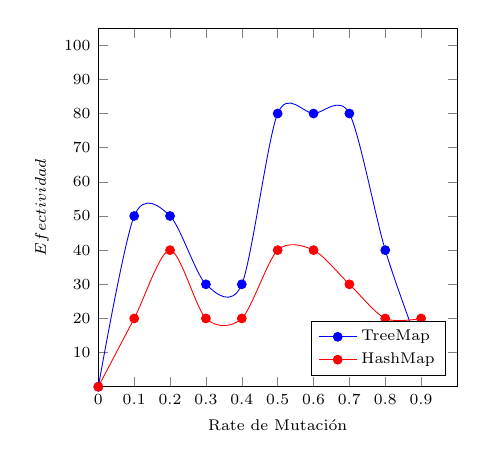
\begin{tikzpicture}[scale=0.8]
\begin{axis}[
    width=0.60\textwidth,
    height=0.60\textwidth,
    xmin=0, xmax=1,
    ymin=0, ymax=105,
    xlabel={\scriptsize{Rate de Mutación}},
    ylabel={\scriptsize{$Efectividad$}},
    xtick={0,0.1,0.2,...,0.9},
    ytick={10,20,...,100},
    legend pos=south east,
    legend cell align={left},
    legend style={font=\scriptsize},
    tick label style={font=\scriptsize}
]

\addplot[mark=*,blue,,smooth] coordinates {
    (0, 0)
    (0.1, 50)
    (0.2, 50)
    (0.3, 30)
    (0.4, 30)
    (0.5, 80)
    (0.6, 80)
    (0.7, 80)
    (0.8, 40)
    (0.9, 10)
};
\addplot[mark=*,red,,smooth] coordinates {
    (0, 0)
    (0.1, 20)
    (0.2, 40)
    (0.3, 20)
    (0.4, 20)
    (0.5, 40)
    (0.6, 40)
    (0.7, 30)
    (0.8, 20)
    (0.9, 20)
};
\legend{TreeMap, HashMap}

\end{axis}
\end{tikzpicture}%
\hfill
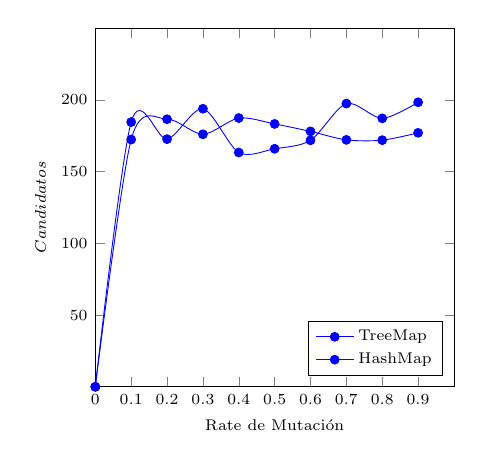
\begin{tikzpicture}[scale=0.8]
\begin{axis}[
    width=0.60\textwidth,
    height=0.60\textwidth,
    xmin=0, xmax=1,
    ymin=0, ymax=250,
    xlabel={\scriptsize{Rate de Mutación}},
    ylabel={\scriptsize{$Candidatos$}},
    xtick={0,0.1,0.2,...,0.9},
    ytick={50,100,150,200},
    legend pos=south east,
    legend cell align={left},
    legend style={font=\scriptsize},
    tick label style={font=\scriptsize}
]

\addplot[mark=*,blue,smooth] coordinates {
    (0,0)
    (0.1, 184.5)
    (0.2, 172.6)
    (0.3, 193.8)
    (0.4, 163.3)
    (0.5, 165.9)
    (0.6, 171.8)
    (0.7, 197.4)
    (0.8, 187.1)
    (0.9, 198.3)
};

\addplot[mark=*,blue,smooth] coordinates {
    (0,0)
    (0.1, 172.3)
    (0.2, 186.5)
    (0.3, 176)
    (0.4, 187.3)
    (0.5, 183.2)
    (0.6, 178)
    (0.7, 172.1)
    (0.8, 171.9)
    (0.9, 177)
};
\legend{TreeMap,HashMap}

\end{axis}
\end{tikzpicture}

\caption{Gráficos de Efectividad y cantidad de candidatos de acuerdo al rate de mutación}
\end{figure}


\begin{figure}
\centering
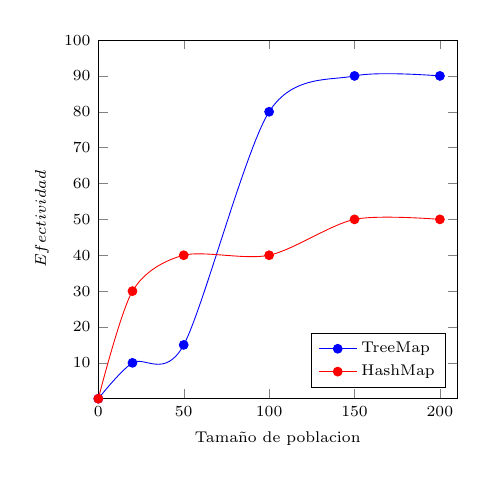
\begin{tikzpicture}[scale=0.8]
\begin{axis}[
    width=0.60\textwidth,
    height=0.60\textwidth,
    xmin=0, xmax=210,
    ymin=0, ymax=100,
    xlabel={\scriptsize{Tamaño de poblacion}},
    ylabel={\scriptsize{$Efectividad$}},
    xtick={0,50,...,200},
    ytick={10,20,...,100},
    legend pos=south east,
    legend cell align={left},
    legend style={font=\scriptsize},
    tick label style={font=\scriptsize}
]

\addplot[mark=*,blue,,smooth] coordinates {
    (0, 0)
    (20, 10)
    (50, 15)
    (100, 80)
    (150, 90)
    (200, 90)

  
};

\addplot[mark=*,red,,smooth] coordinates {
    (0, 0)
    (20, 30)
    (50, 40)
    (100, 40)
    (150, 50)
    (200, 50)

  
};
\legend{TreeMap,HashMap}
\end{axis}
\end{tikzpicture}%
\hfill
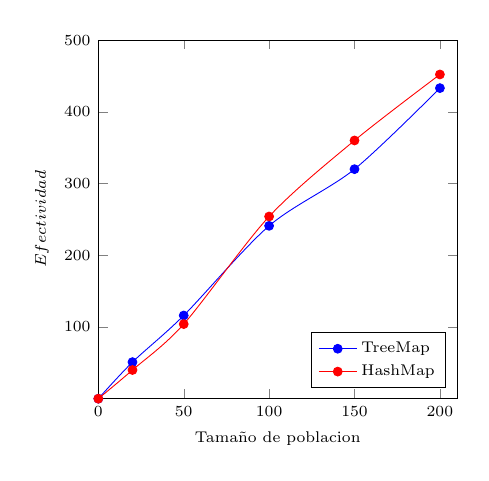
\begin{tikzpicture}[scale=0.8]
\begin{axis}[
    width=0.60\textwidth,
    height=0.60\textwidth,
    xmin=0, xmax=210,
    ymin=0, ymax=500,
    xlabel={\scriptsize{Tamaño de poblacion}},
    ylabel={\scriptsize{$Efectividad$}},
    xtick={0,50,...,200},
    ytick={100,200,...,500},
    legend pos=south east,
    legend cell align={left},
    legend style={font=\scriptsize},
    tick label style={font=\scriptsize}
]

\addplot[mark=*,blue,,smooth] coordinates {
    (0, 0)
    (20, 51)
    (50, 116)
    (100, 241)
    (150, 320)
    (200, 433)

  
};

\addplot[mark=*,red,,smooth] coordinates {
    (0, 0)
    (20, 40)
    (50, 104)
    (100, 254)
    (150, 360)
    (200, 452)

  
};
\legend{TreeMap,HashMap}


\legend{TreeMap, HashMap}

\end{axis}
\end{tikzpicture}

\caption{Gráficos de Efectividad y cantidad de candidatos de acuerdo al rate de mutación}
\end{figure}



\subsubsection{Variacion de acuerdo a los Parametros}

% Ademas, examinamos la sensibilidad de los parámetros del Algoritmo Genético y exploramos los usos de los builders generados. Los resultados obtenidos proporcionaron información valiosa sobre el rendimiento y la utilidad de nuestra técnica en la generación de builders y su aplicación en diversas tareas.


Como vimos en el capitulo \ref{cap:beapi}, necesitamos setear cierto parámetros para el funcionamiento de nuestros algoritmos y nuestras funcion de valoración. Los parametros mas importnate que influyen en la eficiencia y efectividad para nuestro algoritmo geneticos son el \emph{rate} de mutacion y de cross-over y el numero de poblacion y el numero de torneos en la seleccion.
Para nuestra fitness de randoop, es importante saber con cuanto tiempo dispone para generar objectos.
Para la fitness de Beapi, es importante conocer con que scope se llega a una solución optima y eficiente.
Para setear estos valores para la experimentación hemos realizado una tarea de prueba y error para ir viendo con que valores se ajustan mejor nuestros algoritmos. 



mas precisamente \cacho{RefGenetic} para nuestro algoritmo genetico necesitamos setear un \emph{rate} para los operadores geneticos. Para eso hemos probado en los casos de estudios con diferentes valores de cada operador. Nuestra comparacion se basa en medir la cantidad de tiempo que le lleva a cada Algortimo terminar la ejecucio, en la cantidad de candidatos que evalua la funcion de valoracion y cuan bueno es en eficacia para encontrar el minimo y suficiente subconjunto de metodos que pudimos observar en nuestro ground truth \cacho{Agregar seccion}. Ejecutamos el algoritmo 10 veces con el resto de los parametros que no esta en evaluacion con un valor promedio (Crossover=0.5, mutation 0.1, Tournanament 4).
Tambien utilizamos 30 segundos para la fitness con randoop y scope 6 para BEAPI.

En la tabla \ref{tab:CrossOverGA} se puede observar como se comporta el algoritmo cuando se utiliza diferente rate para el operador de CrossOver. 





% \begin{table}[t!]
\centering
\begin{tabular}{l|cc|cc|cc}
\hline

\textbf{Parameters}& \multicolumn{2}{c}{\textbf{Time}} & \multicolumn{2}{c}{\textbf{Candidates}} & \multicolumn{2}{c}{\textbf{Eficacia}} \\
 &RO&BE&RO&BE&RO&BE \\

\hline

0.01 & &  &\\

0.5 & &  &\\
0.1 & &  &\\
0.1 & &  &\\
\midrule

\end{tabular}%
\caption{Diferentes valores de Mutatacion}
\label{tab:MutationGA}
\end{table}

\begin{table}[t!]
\centering
\begin{tabular}{l l ccc}
\hline

\textbf{Parameters}& \textbf{Time} & \textbf{ObjectsCalculate} & \textbf{Eficacia} \\
\midrule

0.01 & &  &\\

0.5 & &  &\\
0.1 & &  &\\
1 & &  &\\
\midrule

\end{tabular}%
\caption{Diferentes valores de mutatacion}
\label{tab:CrossOverGA}
\end{table}

\begin{table}[t!]
\centering
\begin{tabular}{l l ccc}
\hline

\textbf{Parameters}& \textbf{Time} & \textbf{ObjectsCalculate} & \textbf{Eficacia} \\
\midrule

3 & &  &\\

4 & &  &\\
5 & &  &\\
6 & &  &\\
\midrule

\end{tabular}%
\caption{Diferentes valores de Tournaments para seleccion}
\label{tab:SelectionGA}
\end{table}

\subsection{Uso de Builders en verificación}

En el ultimo experimento sobre la identificación de \emph{builders}, utilicé Java PathFinder \cite{Visser:2005} (JPF) para realizar pruebas de generación de entradas de software para estructuras de datos de \emph{java.util}. JPF \cacho{REF} es un verificador de modelos de estado explícito para programas escritos en Java. Para realizar la verificación, las técnicas de versificación de modelos de software se basan en la definición de controladores de métodos: combinaciones de métodos que permiten construir las entradas con las que se ejecutará el programa. Intuitivamente, es deseable seleccionar el menor conjunto de métodos posible, cuyas combinaciones permitan construir todas las estructuras acotadas para el módulo (para analizar el software con todas las entradas posibles). La dificultad de escribir controladores de pruebas es un obstáculo importante para el uso de un verificador de modelos. Esta selección de métodos, que generalmente se realiza manualmente, no es una tarea fácil: requiere un análisis exhaustivo de las rutinas disponibles en el módulo y una comprensión profunda de su semántica.
Es posible construir un método no determinista (harness de test) que genere todas las secuencias de llamadas a métodos de la API hasta un tamaño especificado por el usuario (scope). JPF se utiliza para enumerar todas estas secuencias. JPF almacena todos los estados explorados y retrocede cuando visita un estado previamente explorado.

JPF admite anotaciones de programa que se agregan a los programas a través de llamadas a métodos de una clase especial Verify.
Utilizamos los siguientes métodos de la biblioteca JPF \verb"Verify":
\\
\begin{itemize}
\item El método \verb"Verify.getInt(int lo, int hi)" devuelve un valor entre \verb"lo" y \verb"hi", inclusive. Crea un punto de elección no determinista: JPF necesita explorar las ejecuciones para todos los valores en el rango.
\item \verb"random(int n)" devuelve valores de 0 a \verb"n", de manera no determinista.
\end{itemize}

Si se desea verificar que el método \emph{put}  de TreeMap cumple con el repOK (predicado imperativo que verifica las invariantes de clase) de la estructura de datos, es necesario escribir algo como: 
\\

\begin{lstlisting}[caption={Probando el método put de TreeMap con JPF},label={lst:label},language=Java,captionpos=b]
public static void main(String[] args) {
   int scope = 3;
   TreeMap t = generateStructure(scope);
   t.put(Verify.getInt(0,scope),Verify.getInt(0,scope));
   assert t.repOK();
}
\end{lstlisting}

Para realizar el análisis de esta propiedad, es necesario proporcionar a JPF los mecanismos para generar todo el árbol de entrada (\textit{generateStructure}). 
En el siguiente ejemplo, mostramos un controlador de prueba construido con todos los métodos de la estructura de datos \textit{TreeMap}:
\\
\\
\begin{lstlisting}[caption={Controlador con todos los métodos},label={lst:driverAPI},language=Java,captionpos=b]
private static TreeMap generateStructure(int scope) {
   int maxLength = Verify.getInt(0, scope);
   TreeMap t = new TreeMap();
   for (int i = 1; i <= maxLength; i++) {
      switch (Verify.random(n_methods)) {
         case 0:
            t.put(Verify.getInt(0,scope),Verify.getInt(0,scope));
            break;
         case 1:
            t.remove(Verify.getInt(0,scope));
            break;						
         case 2:
            t.clear();
            break;
         case 3:
            t.containsValue(Verify.getInt(0,scope));
            break;
         ...
         case 11: 
            t.putAll(l);
            break;
      }
   }
   return t;
}
\end{lstlisting}

El método controlador anterior, en primer lugar, selecciona el número de métodos a ejecutar, \textit{maxLength}, un número entre 0 y \textit{scope}. (Linea 2). Cada iteración del ciclo (Linea 4 a 23) corresponde a la ejecución de un solo método, seleccionado de manera no determinista entre todos los disponibles. En el caso de que el usuario no conozca el conjunto de métodos builders (y no quiera hacer el complicado trabajo de seleccionarlos manualmente), la solución más segura para evitar descartar métodos importantes es utilizar todos los métodos disponibles en el módulo, como se muestra en el método controlador descrito anteriormente. En el cuerpo del bucle, a cada método se le asigna un número entero entre 0 y \textit{n\_methods}. Se elige de manera no determinista el método a ejecutar en el ciclo actual. Por ejemplo, si \textit{n\_methods}=1, se ejecuta el método \textit{remove}. Es fácil ver que el número de ejecuciones posibles que se deben explorar por JPF crece exponencialmente con el número de métodos disponibles.

%(for every method that is executed in one iteration, there are \textit{n_methods} possible methods to execute in the next iteration).

Para evitar este crecimiento exponencial en este experimento, se propone utilizar únicamente los constructores detectados por nuestro enfoque explicado en la sección \ref{sec:builders}.
\\
\\
\begin{lstlisting}[caption={Controlador con métodos constructores},label={lst:driverBLD},language=Java,captionpos=b]
private static TreeMap generateStructure(int scope) {
   int maxLength = Verify.getInt(0,scope);
   TreeMap t = new TreeMap();
   for (int i = 1; i <= maxLength; i++) {
      switch (Verify.random(11)) {
         case 0:
            t.put(Verify.getInt(0,scope),Verify.getInt(0,scope));
            break;
         case 1:
            t.remove(Verify.getInt(0,scope));
            break;						
      }
   }
   return t;
}
\end{lstlisting}

Como se muestra en el controlador anterior, solo 2 métodos componen un conjunto mínimo y suficiente para construir controladores para TreeMap de \textit{java.util}. Utilizando solo esos métodos, generamos exactamente los mismos objetos TreeMap que antes (porque los constructores son suficientes y mínimos), y por lo tanto JPF explora las mismas ejecuciones de propiedades con ambos controladores.

Los resultados de la tabla \ref{tab:results1-jpf} y \ref{tab:results2-jpf} muestran que la construcción del controlador a partir de nuestro enfoque presentado permite aumentar la eficiencia y escalabilidad a estructuras más grandes en el análisis utilizando JPF. Esto se debe a la reducción de los métodos utilizados en los controladores (evitando métodos superfluos) y manteniendo la capacidad de construir todos los objetos acotados posibles (debido a la suficiencia de los métodos elegidos) en menos tiempo.




\begin{table}
\scriptsize
\begin{tabular}{ c| l| c c c c c}
\hline
Class & Method & Scope &
\multicolumn{2}{c}{\textsf{Builders}} &
\multicolumn{2}{c}{\textsf{AllMethods}} \\
&&&
\tiny{\textbf{states}} & \tiny{\textbf{time (S)}} &
\tiny{\textbf{states}} & \tiny{\textbf{time (S)} }\\
\hline
\multirow{14}{*}{LinkedList} 
& add
  & 1 & 11  & 0 & 42  & 0 \\
& & 2 & 58  & 0 & 715 & 0 \\
& & 3 & 453 & 0 & 11064 & 2 \\
& & 4 & 4881  & 1 & 153247  & 14  \\
& & 5 & 67183 & 13  & 2291803 & 171 \\
& & 6 & 1120932 & 221 & 39759491  & 2771  \\
& & 7 & 21913097  & 4588  &TO  & \\

\cline{2-7}
 &remove 
  & 1 & 11  & 0 & 42  & 0 \\
& & 2 & 58  & 0 & 715 & 0 \\
& & 3 & 453 & 0 & 11064 & 2\\
& & 4 & 4881  & 1 & 153247  & 14\\
& & 5 & 67183 & 11  & 2291803 & 168\\
& & 6 & 1120932 & 188 & 39759491  & 2713\\
& & 7 & 21913097  & 3998  & TO \\ 

\hline
\multirow{10}{*}{TreeMap} 
% Check
& put
  & 1 & 45  & 0 & 112 & 0 \\
& & 2 & 991 & 0 & 2821  & 0 \\
& & 3 & 16071 & 2 & 71678 & 8 \\
& & 4 & 552807  & 75  & 1757976 & 204 \\
& & 5 & 20601447  & 3007  & TO& \\
\cline{2-7}

& remove
  & 1 & 25  & 0 & 61  & 0 \\
& & 2 & 406 & 0 & 1345  & 0 \\
& & 3 & 8359  & 1 & 33845 & 3 \\
& & 4 & 182732  & 19  & 768564  & 66  \\
& & 5 & 7176075 & 713 & 24775111  & 2341  \\



%  && 5 &  & MO & - & - &MO  &  &-  & -  \\


\hline
\multirow{19}{*}{TreeSet} 
&put
  & 1 & 11  & 0 & 48  & 0 \\
& & 2 & 49  & 0 & 595 & 0 \\
& & 3 & 197 & 0 & 5275  & 1 \\
& & 4 & 806 & 0 & 36427 & 4 \\
& & 5 & 3115  & 0 & 204877  & 19  \\
& & 6 & 12062 & 1 & 1024038 & 90  \\
& & 7 & 47241 & 5 & 4966224 & 452 \\
& & 8 & 501666  & 45  & 23976826  & 2094  \\
& & 9 & 2047285 & 183 &TO  &  \\
\cline{2-7}

& remove
  & 1 & 17  & 0 & 48  & 0 \\
& & 2 & 88  & 0 & 595 & 0 \\
& & 3 & 423 & 0 & 5275  & 1 \\
& & 4 & 1842  & 0 & 36427 & 4 \\
& & 5 & 7455  & 1 & 204877  & 19  \\
& & 6 & 30197 & 3 & 1024038 & 88  \\
& & 7 & 122717  & 10  & 4966224 & 431 \\
& & 8 & 501666  & 43  & 23976826  & 2088  \\
& & 9 & 2047285 & 181 & TO    \\
& & 10  & 8182166 & 719 &    TO  \\
& & 11  & 31473779  & 2738  &  TO     \\
\hline

\end{tabular}%
\caption{Estados generados JPF utilizando el método driver con todos los métodos de la API vs. solo utilizando los métodos builders.}
\label{tab:results1-jpf}
 \end{table}

\begin{table}[!thb]
\scriptsize
\begin{tabular}{ c| l| c c c c c}
\hline
Class & Method & Scope &
\multicolumn{2}{c}{\textsf{Builders}} &
\multicolumn{2}{c}{\textsf{AllMethods}} \\
&&&
\tiny{\textbf{states}} & \tiny{\textbf{time (S)}} &
\tiny{\textbf{states}} & \tiny{\textbf{time (S)} }\\
\hline
\multirow{14}{*}{LinkedList} 
& remove
  & 1 & 17  & 0 & 48  & 0 \\
& & 2 & 88  & 0 & 595 & 0 \\
& & 3 & 423 & 0 & 5275  & 1 \\
& & 4 & 1842  & 0 & 36427 & 4 \\
& & 5 & 7455  & 1 & 204877  & 19  \\
& & 6 & 30197 & 3 & 1024038 & 88  \\
& & 7 & 122717  & 10  & 4966224 & 431 \\
& & 8 & 501666  & 43  & 23976826  & 2088  \\
& & 9 & 2047285 & 181 & TO    \\
& & 10  & 8182166 & 719 &    TO  \\
& & 11  & 31473779  & 2738  &  TO     \\

\hline

\multirow{11}{*}{HM} 
& put
 & 1 & 21& 0& 100 & 0 \\
& & 2 & 136& 0& 235 & 0 \\
& & 3 & 2945& 0& 59494 & 9 \\
& & 4 & 64626& 11&  1808536& 299 \\
& & 5 & 1512217& 267& TO&  \\

 \cline{2-7}

& remove
 & 1 &25 & 0& 56 & 0 \\
& & 2 &325 & 0& 1144 &  0\\
& & 3 & 5479& 1& 23966 & 3 \\
& & 4 & 105607& 10& 627361 &  78\\
& & 5 & 2289075& 213& 22547086 &3011  \\
& & 6 & 55335111 & 5017&TO &  \\

\hline

\multirow{14}{*}{HS} 
& put
  & 1 & 11  & 0 & 30  & 0 \\
& & 2 & 40  & 0 & 248 & 0 \\
& & 3 & 149 & 0 & 1405  & 0 \\
& & 4 & 531 & 0 & 6259  & 1 \\
& & 5 & 1765  & 0 & 24107 & 3 \\
& & 6 & 5496  & 0 & 84617 & 8 \\
& & 7 & 16217 & 2 & 278241  & 24  \\


\cline{2-7}

& remove
  & 1 & 11  & 0 & 30  & 0 \\
& & 2 & 40  & 0 & 248 & 0 \\
& & 3 & 149 & 0 & 1405  & 0 \\
& & 4 & 531 & 0 & 6259  & 1 \\
& & 5 & 1765  & 0 & 24107 & 3 \\
& & 6 & 5496  & 0 & 84617 & 8 \\
& & 7 & 16217 & 1 & 278241  & 24  \\

\hline

\end{tabular}%
\caption{Estados generados JPF utilizando el método driver con todos los métodos de la API vs. solo utilizando los métodos builders.}
\label{tab:results2-jpf}
 
\end{table}













\begin{table}[!thb]
\scriptsize

\centering
\begin{tabular}{ l r | r | r | r | r  }
  \toprule
  \multicolumn{6}{c}{\textbf{Real World}} \\
  \midrule 
  \textbf{Class} & \textbf{S} & \textbf{SM/BLD} & \textbf{SM}  & \textbf{BLD} & \textbf{NoOPT}  \\
  \midrule
  NCL
  & 3 & .10 & .47 & -  & -  \\
  & 4 & .41 & 3.48  &  - & -  \\
  & 5 & 3.33  &  - &  - & -  \\
  & 6 & 73.78 &  - &  - &  - \\
  \midrule
  TSet
  & 3 & .03 & .07 & 56.82 & - \\
  & 11  & 21.52 & 86.06 &  - & -  \\
  & 12  & 69.98 & 276.85  &  - & -  \\
  & 13  & 226.66  & 887.83  &  - & -  \\
    \midrule
  TMap
  & 3 & .11 & .25 & - & - \\
  & 4 & .75 & 2.36  &  - &  - \\
  & 5 & 15.97 & 57.64 &  - & -  \\
  & 6 & 839.87  & 2901.37 &  - &  - \\
  \midrule
  LList
  & 3 & .02 & .13 & .64 & - \\
  & 6 & .96 & 258.85  & -  &  - \\
  & 7 & 12.98 &  - &  - &  - \\
  & 8 & 286.21  & -  & -  & -  \\
  \midrule
  HMap
  & 3 & .10 & 11.49 & - & - \\
  & 4 & .55 & -  & -  & -  \\
  & 5 & 5.33  & -  &  - &  - \\
  & 6 & 119.87  &  - &  - &  - \\
  \bottomrule

\end{tabular}

\label{table:beapi}

\end{table}

